% \begin{figure}[H]
% \centering
% \begin{subfigure}{.5\textwidth}
%   \centering
%   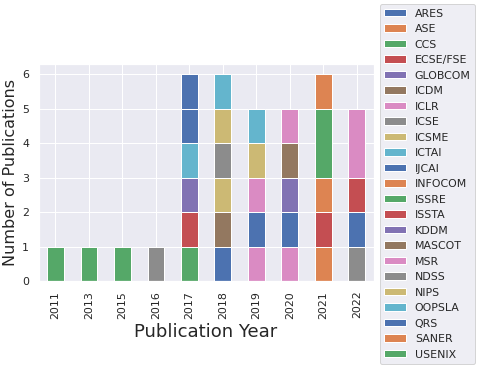
\includegraphics[width=0.9\linewidth]{Figures/RQ1/distribution_conf.png}
%   \caption{Number of studies published in various conferences.}
%   \label{fig:venue1}
% \end{subfigure}%
% \begin{subfigure}{.5\textwidth}
%   \centering
%   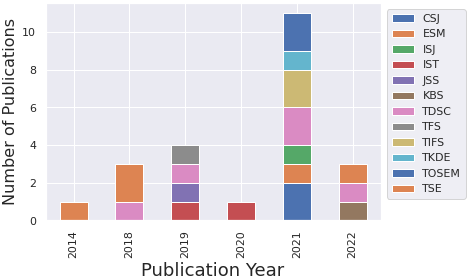
\includegraphics[width=1.2\linewidth]{Figures/RQ1/distribution_jour.png}
%   \caption{Number of studies published in various journals.}
%   \label{fig:venue2}
% \end{subfigure}%
% \newline
% \caption{Distribution of different publication venues.}
% \label{fig:pub_venues}
% \end{figure}

       %  xticklabels={ {ARES}, {ASE}, {CCS}, {ECSE/FSE}, {GLOBCOM}, {ICDM}, {ICLR},
       % {ICSE}, {ICSME}, {ICTAI}, {IJCAI}, {INFOCOM}, {ISSRE}, {ISSTA},
       % {KDDM}, {MASCOT}, {MSR}, {NDSS}, {NIPS}, {OOPSLA}, {QRS}, {SANER},
       % {USENIX}},
% \definecolor{ForestGreen}{RGB}{34,139,34}
% \pgfplotstableread{
% PublicationYear	2011 	2013 	2015 	2016 	2017 	2018 	2019 	2020 	2021 	2022
% ASE 	0 	0 	0 	0 	0 	0 	0 	0 	1 	0
% CCS 	0 	1 	1 	0 	1 	0 	0 	0 	0 	0
% ECSE/FSE 	0 	0 	0 	0 	1 	0 	0 	0 	1 	0
% ICDM 	0 	0 	0 	0 	0 	1 	0 	0 	0 	0
% ICLR 	0 	0 	0 	0 	0 	0 	1 	1 	0 	0
% ICSE 	0 	0 	0 	1 	0 	0 	0 	0 	0 	1
% IJCAI 	0 	0 	0 	0 	1 	0 	1 	1 	0 	1
% INFOCOM 	0 	0 	0 	0 	0 	0 	0 	0 	1 	0
% ISSTA 	0 	0 	0 	0 	0 	0 	0 	0 	0 	1
% NDSS 	0 	0 	0 	0 	0 	1 	0 	0 	0 	0
% NIPS 	0 	0 	0 	0 	0 	1 	1 	0 	0 	0
% OOPSLA 	0 	0 	0 	0 	0 	1 	1 	0 	0 	0
% USENIX 	1 	0 	0 	0 	0 	0 	0 	0 	0 	0
% }\testdata
% \begin{figure}[t!]
% \centering
% \renewcommand{\arraystretch}{1}
% \resizebox{0.6\columnwidth}{!}{%
%     \begin{tikzpicture}[scale=0.6]
%     \begin{axis}[
%         ybar stacked,
%     	bar width=15pt,
%         ymin=0,
%         ymax=5,
%         xtick=data,
%         legend style={at={(1.01,0.6)},anchor=west},
%         reverse legend=true,
%         %yticklabels from table={\testdata}{Label},
%         xticklabels={ {ASE}, {CCS}, {ECSE/FSE}, {ICDM}, {ICLR}, {ICSE}, {IJCAI},
%        {INFOCOM}, {ISSTA}, {NDSS}, {NIPS}, {OOPSLA},{USENIX}},
%         xticklabel style={rotate=25,anchor=east},
%     ]
%     \addplot + [ nodes near coords, fill=green!80]      table    [y=2011, meta=Label, x expr=\coordindex] {\testdata};
%     \addplot + [nodes near coords, fill=blue!60]         table    [y=2013, meta=Label, x expr=\coordindex] {\testdata};
%     \addplot + [nodes near coords, fill=red!60]         table    [y=2015, meta=Label, x expr=\coordindex] {\testdata};
%     \addplot + [nodes near coords, fill=ForestGreen!60] table    [y=2016, meta=Label, x expr=\coordindex] {\testdata};
%     \addplot + [nodes near coords, fill=yellow!60]      table    [y=2017, meta=Label, x expr=\coordindex] {\testdata};
%     \addplot + [nodes near coords, fill={rgb:red,1;green,2;blue,5}] table [y=2018, meta=Label, x expr=\coordindex] {\testdata};
%     \addplot + [nodes near coords, fill={rgb:blue,1;yellow,2;pink,5}] table    [y=2019, meta=Label, x expr=\coordindex] {\testdata};
%     \addplot + [nodes near coords, fill={rgb:yellow,1;red,2;pink,5}] table    [y=2020, meta=Label, x expr=\coordindex] {\testdata};
%     \addplot + [nodes near coords, fill={rgb:pink,1;yellow,2;orange,5}] table    [y=2021, meta=Label, x expr=\coordindex] {\testdata};
%     \addplot + [nodes near coords, fill={rgb:orange,1;blue,2;pink,5}] table    [y=2022, meta=Label, x expr=\coordindex] {\testdata};
% \legend{2011,
% 2013,
% 2015,
% 2016,
% 2017,
% 2018,
% 2019,
% 2020,
% 2021,
% 2022
% }
% \end{axis}
% \end{tikzpicture}}
% \caption{The distribution of software vulnerabilities in the studied ML libraries.}
% \label{typeDist}
% \end{figure}

\definecolor{airforceblue}{rgb}{0.36, 0.54, 0.66}
\definecolor{aliceblue}{rgb}{0.94, 0.97, 1.0}
\definecolor{alizarin}{rgb}{0.82, 0.1, 0.26}
\definecolor{almond}{rgb}{0.94, 0.87, 0.8}
\definecolor{amaranth}{rgb}{0.9, 0.17, 0.31}
\definecolor{amber}{rgb}{1.0, 0.75, 0.0}
\definecolor{amber(sae/ece)}{rgb}{1.0, 0.49, 0.0}
\definecolor{americanrose}{rgb}{1.0, 0.01, 0.24}
\definecolor{amethyst}{rgb}{0.6, 0.4, 0.8}
\definecolor{anti-flashwhite}{rgb}{0.95, 0.95, 0.96}
\definecolor{antiquebrass}{rgb}{0.8, 0.58, 0.46}
\definecolor{antiquefuchsia}{rgb}{0.57, 0.36, 0.51}



% \pgfplotstableread{
% ASE	ICLR	USENIX	ISSRE	SANER	IJCAI	ICSME	ISSTA	ICDM	ICTAI	ARES	MSR	OOPSLA	CCS	NIPS	ICSE	ECSE/FSE
% 2020 0	1	0	0	0	1	0	0	0	0	0	1	0	0	0	0	0
% 2013 0	0	0	0	0	0	0	0	0	0	0	0	0	1	0	0	0
% 2022 1	0	0	0	0	1	0	1	0	0	0	2	0	0	0	1	2
% 2011 0	0	1	0	0	0	0	0	0	0	0	0	0	0	0	0	0
% 2018 0	0	0	0	0	0	1	0	1	0	1	0	1	0	1	0	0
% 2015 0	0	0	0	0	0	0	0	0	0	0	0	0	1	0	0	0
% 2021 1	0	0	2	1	0	0	0	0	0	0	0	0	0	0	0	1
% 2019 0	1	0	0	0	1	0	0	0	0	0	1	1	0	1	0	0
% 2017 0	0	0	0	0	1	0	0	0	1	0	0	0	1	0	0	1
% 2016 0	0	0	0	0	0	0	0	0	0	0	0	0	0	0	1	0
% }\testdata
% \begin{figure}[H]
% \centering
% \begin{subfigure}{.5\textwidth}
% \centering
% \begin{tikzpicture}[scale=0.6]
% \begin{axis}[
%         ybar stacked,
%     	bar width=15pt,
%         ymin=0,
%         ymax=5,
%         xtick=data,
%         legend style={at={(1.01,0.54)},anchor=west},
%         reverse legend=true,
%         %yticklabels from table={\testdata}{Label},
%         xticklabels={ {2011}, {2013}, {2015}, {2016}, {2017}, {2018}, {2019},
%        {2020}, {2021}, {2022}},
%         xticklabel style={rotate=25,anchor=east},
%     ]
%     \addplot + [ nodes near coords, fill=green!80]      table    [y=ASE, meta=Label, x expr=\coordindex] {\testdata};
%     \addplot + [nodes near coords, fill=blue!60]         table    [y=CCS, meta=Label, x expr=\coordindex] {\testdata};
%     \addplot + [nodes near coords, fill=red!60]         table    [y=ECSE/FSE, meta=Label, x expr=\coordindex] {\testdata};
%     \addplot + [nodes near coords, fill=ForestGreen!60] table    [y=ICDM, meta=Label, x expr=\coordindex] {\testdata};
%     \addplot + [nodes near coords, fill=yellow!60]      table    [y=ICLR, meta=Label, x expr=\coordindex] {\testdata};
%     \addplot + [nodes near coords, fill={antiquefuchsia}] table [y=ICSE, meta=Label, x expr=\coordindex] {\testdata};
%     \addplot + [nodes near coords, fill={airforceblue}] table    [y=IJCAI, meta=Label, x expr=\coordindex] {\testdata};
%     \addplot + [nodes near coords, fill={aliceblue}] table    [y=INFOCOM, meta=Label, x expr=\coordindex] {\testdata};
%     \addplot + [nodes near coords, fill={alizarin}] table    [y=ISSTA, meta=Label, x expr=\coordindex] {\testdata};
%     \addplot + [nodes near coords, fill={almond}] table    [y=NIPS, meta=Label, x expr=\coordindex] {\testdata};
%     \addplot + [nodes near coords, fill={amaranth}] table    [y=OOPSLA, meta=Label, x expr=\coordindex] {\testdata};
%     \addplot + [nodes near coords, fill={amber}] table    [y=USENIX, meta=Label, x expr=\coordindex] {\testdata};
% \legend{ASE,
% CCS,
% ECSE/FSE,
% ICDM,
% ICLR,
% ICSE,
% IJCAI,
% INFOCOM,
% ISSTA,
% NIPS,
% OOPSLA,
% USENIX
% }
% \end{axis}
% \end{tikzpicture}
% \caption{Number of studies published in various conferences.}
% \label{fig:venue1}
% \end{subfigure}%
% \pgfplotstableread{
% PublicationYear TFS	TKDE TOSEM TSE
% 2014 	0 	0 	0 	1
% 2018 	0 	0 	0 	2
% 2019 	1 	0 	0 	0
% 2021 	0 	1 	2 	0
% 2022 	0 	0 	0 	1
% }\testdata
% \begin{subfigure}{.5\textwidth}
% \centering
% \begin{tikzpicture}[scale=0.6]
% \begin{axis}[
%         ybar stacked,
%     	bar width=15pt,
%         ymin=0,
%         ymax=5,
%         xtick=data,
%         legend style={at={(1.01,0.54)},anchor=west},
%         reverse legend=true,
%         %yticklabels from table={\testdata}{Label},
%         xticklabels={ {2014}, {2018}, {2019}, {2021}, {2022}},
%         xticklabel style={rotate=25,anchor=east},
%     ]
%     \addplot + [ nodes near coords, fill=green!80]      table    [y=TFS, meta=Label, x expr=\coordindex] {\testdata};
%     \addplot + [nodes near coords, fill=blue!60]         table    [y=TKDE, meta=Label, x expr=\coordindex] {\testdata};
%     \addplot + [nodes near coords, fill=red!60]         table    [y=TOSEM, meta=Label, x expr=\coordindex] {\testdata};
%     \addplot + [nodes near coords, fill=ForestGreen!60] table    [y=TSE, meta=Label, x expr=\coordindex] {\testdata};
% \legend{TFS,
% TKDE,
% TOSEM,
% TSE
% }
% \end{axis}
% \end{tikzpicture}
% \caption{Number of studies published in various journals.}
% \label{fig:venue2}
% \end{subfigure}%
% \newline
% \caption{Distribution of different publication venues.}
% \label{fig:pub_venues}
% \end{figure}


